\documentclass[a4paper, 11pt]{article}

% \usepackage{bytefield}
\usepackage{enumitem}
\usepackage{changelog}
\usepackage[hidelinks]{hyperref}
\usepackage[T1]{fontenc}
\usepackage{siunitx}
% \sisetup{text-family-to-math = true, text-series-to-math = true, group-separator = {,}}
\usepackage[ main=english,]{babel}
%% These additional packages are used within the document:
\usepackage{booktabs}  % Tables
\usepackage{multirow}
\usepackage{tabularx}
\usepackage{tikz}      % Diagrams
\usetikzlibrary{arrows, calc, shapes, backgrounds, shadows, positioning}
\usetikzlibrary{fit}
\usetikzlibrary{patterns}

\tikzstyle{int}=[draw, fill=blue!20, minimum size=2em]
\tikzstyle{init} = [pin edge={to-,thin,black}]
\tikzstyle{bits} = [font=\footnotesize]
\usepackage{pgf}
\usepackage{pgf-umlsd}
\usepackage[utf8]{inputenc}
\usepackage{lipsum}
\usepackage{xspace}
\usepackage{calc}


\setlength{\marginparwidth}{1.5cm}
\usepackage{todonotes}
% \usepackage{natbib}
\usepackage{csquotes}
\usepackage[nolist]{acronym}

\usepackage[backend=biber, style=ieee, sortcites, maxcitenames=1,mincitenames=1]{biblatex}
\AtEveryBibitem{
   \clearfield{month}
   \clearfield{series}
%    \clearfield{venue}
   \clearname{editor}
   \clearlist{publisher}
   \clearlist{location} % alias to field 'address'
   \clearfield{eprint}
   \clearfield{doi}
%    % \clearfield{url}
   % \clearfield{venue}
   \clearfield{issn}
   \clearfield{isbn}
   \clearfield{note}
%    \clearfield{urldate}
%    \clearfield{urlday}
%    \clearfield{urlmonth}
%    \clearfield{urlyear}
   \clearfield{eventdate}
   \clearfield{pages}
   \clearlist{language}
   % \clearfield{booktitle}
   % \clearfield{journaltitle}
   \clearfield{volume}
    \ifentrytype{article}{
      \clearfield{number}
      \clearfield{url}
      \clearfield{urlday}
      \clearfield{urlmonth}
      \clearfield{urlyear}
  }{}
    \ifentrytype{inproceedings}{
      \clearfield{number}
      \clearfield{url}
      \clearfield{urlday}
      \clearfield{urlmonth}
      \clearfield{urlyear}
  }{}
}


\usepackage{stackrel}
\usepackage{amsmath, amssymb}
\usepackage{nicefrac}

\usepackage{float}
\floatstyle{plain}
\newfloat{lstfloat}{tpbh}{lop}
\floatname{lstfloat}{Listing}
\def\lstfloatautorefname{Listing}

\usepackage{xurl}       % `\url`s
\usepackage{listings}  % Code listings

\usepackage{tablefootnote}
\usepackage{pifont}


\lstset{%
  basicstyle=\small\ttfamily,
  breakatwhitespace=false,
  breaklines=true,
  commentstyle=\color{green!60!black},
  extendedchars=true,
  keywordstyle=\color{blue},
  showspaces=false,
  showstringspaces=false,
  showtabs=false,
  stringstyle=\color{violet},
  numberstyle=\tiny\color{gray},
  numbers=left,
  numbersep=5pt,
  frame=single,
  tabsize=2,
}
% Fix space after caption,
% see https://tex.stackexchange.com/questions/248804/ieee-latex-listing
\makeatletter
\def\lst@makecapton{%
  \def\@captype{table}%
  \@makecaption
}
\makeatother

% \usepackage{fontawesome5}

% Crypto stuff
% \usepackage{algorithm}
\usepackage[ n, advantage, operators, sets, adversary, landau, probability,
notions, logic, ff, mm, primitives, events, complexity, asymptotics, keys,
% oracles
]{cryptocode}
% \usepackage{algpseudocode}
\usepackage{algorithmicx}

\usepackage[capitalise]{cleveref}
\crefname{enumi}{}{}

\newcommand{\authnote}[2]{{\bf \textcolor{blue}{#1}: \em \textcolor{red}{#2}}}

\newenvironment{packeditemize}{
\begin{list}{$\bullet$}{
\setlength{\itemsep}{1.5pt}
\setlength{\labelwidth}{8pt}
\setlength{\leftmargin}{10pt}
\setlength{\labelsep}{3pt}
\setlength{\listparindent}{\parindent}
\setlength{\parsep}{1.5pt}
\setlength{\parskip}{1.5pt}
\setlength{\topsep}{1.5pt}}}{\end{list}}

\addbibresource{bibliography.bib}

\graphicspath{{figures/}}

%-------------------------------------------------------------------------------
\begin{document}

%-------------------------------------------------------------------------------
\begin{acronym}
\acro{AGPL}{GNU Affero General Public License version 3.0}
\acro{DH}{Diffie-Hellman}
\acro{KDF}{key derivation function}
\acro{MITM}{Machine-in-the-middle}
\acro{OT}{Operational Transformation}
\acro{SP}{Security Property} \acroplural{SP}[SPs]{Security Properties}
\acro{TLS}{Transport Layer Security}
\acro{XHR}{XMLHttpRequest}
\end{acronym}

\author{Theo von Arx and Aaron MacSween}

\title{Security Recommendations for CryptPad 5}

\maketitle

\tableofcontents

\section{Introduction}

  During the writing of the cryptography white paper, we discovered multiple issues and limitations in the current version of CryptPad.
  While none of them are classified severe, requiring immediate action, or posing a serious threat for users, they nevertheless should be addressed.

  In this document, we list the problems, show their consequences, suggest how to fix them and outline possible drawbacks.
  We classified them into three different categories: short-term improvements (c.f. \cref{sec:shortterm}) that can be done immediately within the current version of CryptPad, mid-term improvements (c.f. \cref{sec:midterm}) that require the introduction of a new version of the encryption schemes, and long-term improvements (c.f. \cref{sec:longterm}) that can only be addressed with architectural changes.


\section{Short-Term Improvements} \label{sec:shortterm} % Can be done within current system
  In this section, we list improvements that can be done without requiring bigger changes of the underlying encryption schemes or architecture.

  \subsection{Update TweetNaCl}

\paragraph{Problem:} CryptPad uses TweetNaCl~\cite{Bernstein2015,Chestnykhm2016} version~0.12.2 (September 18, 2014) while the newest version is 1.0.3 (February 10, 2020).

\paragraph{Consequences:} CryptPad misses optimizations and security fixes introduced in later versions.
In the current version, \texttt{nacl.sign} or \texttt{nacl.sign.detached} could create incorrect signatures.
Moreover, CryptPad it might be hard to update TweetNaCl in case of a severe security issue.

\paragraph{Suggestions:} Update TweetNaCl to the latest version.

\paragraph{Drawbacks:}
TweetNaCl has refactored some of the utilities into a separate library and now properly validates the base64 padding before decoding.
An update therefore requires significant work.

  \subsection{Name of Team Roles}

\paragraph{Problem:}
The four roles in a team are called \textit{viewer}, \textit{member}, \textit{admin}, and \textit{owner}.
The role \textit{member} conflicts with the common notion of \enquote{being a member of a team}.

\paragraph{Consequences:}
Users are confused about the difference and precise wording in documentations is difficult.

\paragraph{Suggestions:}
Replace \textit{member} with \textit{author}.

\paragraph{Drawbacks:}
The notion of an \textit{author} may not smoothly match the context of creating folders or drawing in a whiteboard.

  \subsection{Thumbnails of Destroyed Documents}

\paragraph{Problem:}
When an image is destroyed, the thumbnail can be restored using the history function.

\paragraph{Consequences:}
The image is not fully deleted which is not what users expect.

\paragraph{Suggestions:}
When destroying an image, also destroy the thumbnail. In case that the thumbnail is needed to browse the history of a folder, replace the thumbnail with a generic one.

\paragraph{Drawbacks:} -

  \subsection{Asynchronous Cryptography Functions}

\paragraph{Problem:}
The current cryptography functions including encryption and key derivation (such as \texttt{ViewCryptor2}) are synchronous and do block all resources.

\paragraph{Consequences:}
No operations can be done in parallel to cryptography functions.
Moreover, natively supported asynchronous functions (e.g., \texttt{SHA-256}) that would bring a speedup cannot be used.

\paragraph{Suggestions:}
Opt for a more general interface in which cryptography functions are asynchronous

\paragraph{Drawbacks:}
The additional workload coming from parallel execution may be too resource-intensive on some devices, such as smartphones.
Refactoring large parts of the code to make it asynchronous is tedious.

  \subsection{Enforcing of Self-Destructing Links}

\paragraph{Problem:}
The destroying of a document that was shared with a \textit{view-once-and-destroy} is not enforced by the server.

\paragraph{Consequences:}
A malicious user can open such a link, but decide to not destroy the document.
However, it is hard to come up with a scenario in which a malicious user could not achieve the same by simply taking a screenshot of the document.

\paragraph{Suggestions:}
Enforce the destruction on the server side.

\paragraph{Drawbacks:} Although the server sent the content, there is no guarantee that the user actually received it (e.g., due to connectivity problems or an active network attack).
Hence a document could get destroyed before being accessed the first time.\footnote{Currently, a destroyed document is only achieved, and could therefore be restored by instance admins).}

  \subsection{Contact Verification}

\paragraph{Problem:}
There is no easy way to verify whether a CryptPad contact corresponds to the expected person.
Profile pages contain the public key of the users, but they are not signed and hence spoofable.

\paragraph{Consequences:}
Attackers can impersonate a person and gain access to teams, documents and folders.

\paragraph{Suggestions:}
Implement a method that allows users to verify their contacts and whether a conversation is secure.
One approach could be to use safety numbers~\cite{Marlinspike2016} to let users verify whether the binding of the public key to the user is correct.
It is important to provide a clean interface that is easily understandable for users and invites them to actually perform the contact verification.

\paragraph{Drawbacks:} -

  \subsection{Prevent replay of old patches}

\paragraph{Problem:}
Malicious users with read access can replay old patches drafted by other users.
Since they have a valid signatures, they will be accepted.

\paragraph{Consequences:}
Malicious users can send old checkpoints and thus reset documents.
Malicious users could also generate a lot of traffic which might result in a \ac{DoS}.

\paragraph{Suggestions:}
There are multiple approaches:
\begin{enumerate}
  \item Add a time stamp to patches and accept them only if they are within a certain range to the current time.
    The time stamps must be in the signed part of the message to make them unforgeable.
  \item The server keeps a list of the hash of the last $N$ accepted messages.
    Every incoming message is valid if its hash is not in the list and if it references the hash of one of messages in the list.
  \item Clients that want to send patches have to first prove to the server that they are allowed to do so.
    For that, the server sends them a random value (a \textit{challenge}) which they must sign and return.
    If they succeed, they are marked to have write capabilities and the server accepts their patches.
\end{enumerate}

\paragraph{Drawbacks:}
The drawbacks for the different approaches are the followings:
\begin{enumerate}
  \item Users with a wrong system time won't be able to produce new patches.
  \item
    \begin{itemize}
      \item The mechanism is fairly complex for the server and $N$ has to be chosen carefully, and dependent of the number of users with right access (the more there are, the bigger the chance of simultaneous messages that could result in missing the window).
      \item Some types of data structures built on top of channels (such as mailboxes) contain sequences of messages which are independent of each other.
        For these types of channels it could be inconvenient to have to know the parent patch.
        Replay protection could therefore be enforced selectively with an attribute set in the channel metadata.
    \end{itemize}
  \item The challenge/verification has to be s.t. a \ac{DoS} attack (state exhaustion) against the server is not possible.
\end{enumerate}


  \subsection{Concurrent Uploads}

\todo[inline]{TODO: Aaron}

\paragraph{Problem:}

\paragraph{Consequences:}

\paragraph{Suggestions:}

\paragraph{Drawbacks:}

  \subsection{More Entropy for Login Keys}

\paragraph{Problem:}
Generally, neither the username nor the password provides good entropy.
The only rule imposed on the password is that it should have a minimum length of 8 characters.
Therefore, weak passwords such as \texttt{password} are accepted.

\paragraph{Consequences:}
We use \texttt{Scrypt(password, username + InstanceSalt)} to generate the login keys (master keys).
Since these master keys are not generated from a good source of randomness, attackers can gain access to all documents of users with weak passwords.

A side consequence is that the probability to register a new account with the same \texttt{username} and \texttt{password} combination is not negligible. If this happens, then users without bad intentions get access to a third person's drive.

\paragraph{Suggestions:}
Use password strength estimation such as \texttt{zxvbn-ts}~\cite{Wheeler2016,MrWook2022} which rates the password strength on a score from 0 to 4 and provides, guessing times, indicators what makes the password weak and how it can be improved (see \cref{fig:zxvbn}).
We may display the password strength estimation and/or require a minimum score.


\begin{figure}[t]
  \centering
  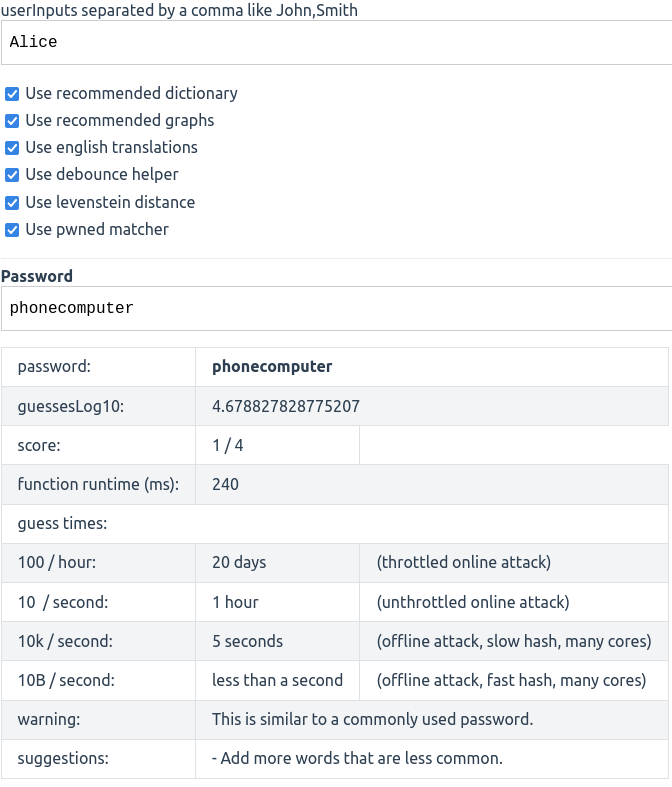
\includegraphics[width=0.55\columnwidth]{images/zxvbn.png}
  \caption{The library \texttt{zxvbn-ts} provides a score, guess times, warnings, and suggestions.}
  \label{fig:zxvbn}
\end{figure}

\paragraph{Drawbacks:} Users are annoyed by password requirements.

  \subsection{Limit Login Block Size}

\paragraph{Problem:}
There is no maximum login block size enforced by the server.

\paragraph{Consequences:}
Attackers can run a \ac{DoS} attack on the server's memory by uploading large data as login blocks.
The initial login block has to be signed which may impose too much computational work for the attack to be successful.
However, the initial login block can be replaced in which case only the corresponding public key has to be signed.

\paragraph{Suggestions:}
Impose a limit on the login block size.

\paragraph{Drawbacks:}
The username is part of the login block. Therefore the size is not bound theoretically, but only practically (e.g., username not bigger than 100 characters).\footnote{It is unclear, whether the username is needed to be in the login block at all. This has to be further investigated.}
Moreover, the login block size might grow in the future in which case the limit has potentially to be adapted.

  \subsection{Instance salt is rarely set}

\paragraph{Problem:}
Instance administrators need to set a custom \texttt{loginSalt} before running CryptPad in a production environment.
This value is supposedly only rarely changed from the default.

\paragraph{Consequences:}
The \texttt{loginSalt} makes it such attackers who want to brute-force common credentials must do so again on each CryptPad instance that they wish to attack. If \texttt{loginSalt} is the default one, then there is no protection against this.

\paragraph{Suggestions:}
\begin{enumerate}
  \item Mention the \texttt{loginSalt} more prominently in the documentation.
  \item Write an installation script that initializes this salt to a random value.
\end{enumerate}

\paragraph{Drawbacks:}


\section{Medium-Term Improvements} \label{sec:midterm} % Can be done within a new Crypto version
  In this section, we outline improvements that should be addressed with the introduction of a new version of the encryption scheme.
  \subsection{Fix Bit Overlap in ViewCryptor2}

\paragraph{Problem:}

In the function \href{https://github.com/xwiki-labs/chainpad-crypto/blob/c8b76b895f67719a3b799daac3d832fdfea45613/crypto.js#L206-L214}{\texttt{createViewCryptor2}}, there is a bit overlap of 128 when generating a symmetric key and a signing key pair.

\paragraph{Consequences:}
An adversary having only access to one of the keys has better chances to guess the other one.
Since there are still 128 independent bits, the vulnerability is not considered severe, but should be fixed in a future version.

\paragraph{Suggestions:}
There are several ways to resolve the issue:
\begin{enumerate}
  \item Increase the size of the seed to have enough bits to make the keys independent.
  \item Hash bytes 16 to 64 to get again a string of 64 bytes.
  \item Use a \href{https://git.xwikisas.com/xwiki-labs/blueprints/-/blob/8ade62e6245dd6d39106ac91376886bafa9ca9c5/prng.js}{consumer-based programming pattern} (similarly as it is already done for \href{https://github.com/xwiki-labs/cryptpad/blob/ce56447031c7644d87d802d5f5b22afbc7b7b923/www/common/common-credential.js#L50-L86}{the credentials}) that can produce \enquote{infinitely} many pseudo-random bytes.
    This essentially hinders us from making such mistakes in the futures.
\end{enumerate}

\paragraph{Drawbacks:}
This requires to introduce a new version of encryption while keeping the old one for backwards compatibility.

  \subsection{Deduplicate Code}

\paragraph{Problem:}
The functions \href{https://github.com/xwiki-labs/chainpad-crypto/blob/c8b76b895f67719a3b799daac3d832fdfea45613/crypto.js#L191}{\texttt{createViewCryptor2}} and \href{https://github.com/xwiki-labs/chainpad-crypto/blob/c8b76b895f67719a3b799daac3d832fdfea45613/crypto.js#L276}{\texttt{createFileCryptor2}} essentially provide the same functionality:
provide a read-only access to a document.

\paragraph{Consequences:}
It is harder to understand and maintain what the two functions do.

\paragraph{Suggestions:}
Merge the two functions and make them callable with and without a \myAlgofont{keyStr}.

\paragraph{Drawbacks:}
The \mychanID of \texttt{createViewCryptor2} is 16 bytes long, while the one of \texttt{createFileCryptor2} has 24 bytes.
Furthermore, \texttt{createFileCryptor2} does not use the secondary signing key pair that is produced by \texttt{createViewCryptor2}.

  \subsection{Transition to New Encryption Schemes}

\paragraph{Problem:}
When a new CryptPad versions introduces new encryption scheme, old documents are not updated to this.

\paragraph{Consequences:}
If a vulnerability in the encryption scheme is discovered, old documents can not be protected other than being destroyed. To keep the content, users would need to manually export and import it.

\paragraph{Suggestions:}
Implement an upgrade mechanism to the latest encryption scheme that can be activated by users.
Ideally, the old links are still valid.
To achieve this, the new keys can be generated from the same seed as the old ones and the old URL can redirect to the new one.

\paragraph{Drawbacks:}
Users might get confused, and old links may be broken after the upgrade.


\section{Long-Term Improvements} \label{sec:longterm} % Require a new architecture
  In this section, we discuss improvements that require an architectural change to address the underlying problems.
  \subsection{Reduce Trust on Server}

\paragraph{Problem:}
Users have to trust the server to deliver the correct client code.

\paragraph{Consequences:}
The threat model is reduced to a honest-but-curious server.
Without the limitation of trusting correct client code delivery, CryptPad could defend against an attacker with more active capabilities.

\paragraph{Suggestions:}
There are multiple approaches:
\begin{enumerate}
  \item Providing an API so that a client can be distributed over an independent channel (App-store, GitHub, Browser extensions, ...).
  \item Trust on First Use (TOFU): users are warned when their client code changes and are asked whether they want to accept the update or not.
  \item Sign the client code and allow users to verify the signature.
\end{enumerate}

\paragraph{Drawbacks:}
\begin{enumerate}
  \item It gets more complicated to use CryptPad, when users first need to download a client. Hence, the webclient should still be accessible.
  \item Currently, all users have the same client version. If this is no more the case, there might be incompatible features, or even \enquote{client fights}, i.e., clients are resolving patches differently and thus always trying to push their version of the document.
  \item Some measures such as signed code may only be effective if the users verify them. As experience in the context of HTTPS verification with extended validation have shown~\cite{Keizer2019}, this might not be the case.
  \item The code should not only be verified for the flagship instance, but also for custom instances. However, they might want to customize the client code.
\end{enumerate}

  \subsection{Team Key Revocation}

\paragraph{Problem:}
The keys of team drives are static and will never change.

\paragraph{Consequences:}
Once a user is kicked from a team, the user does not lose the keys.
Since are not prevented from subscribing to any Netflux channel, they can still receive all messages and also decrypt them with their kept keys.
Hence, they do technically not lose access to the team drive.

\paragraph{Suggestions:}
When someone is kicked from a team, the admin has to automatically create a new key pair and distribute it \textit{privately} to all members.

\paragraph{Drawbacks:} -

  \subsection{Traitor Tracing}

\paragraph{Problem:}
Everyone having read/write access to a document or folder can forward the keys without being noticed by anyone else.

\paragraph{Consequences:}
The access to folders and documents can be delegated without being noticed.
As such team members have partial admin rights since they can share (but not deny) access to documents.

There is currently no way to find who leaked a document.

\paragraph{Suggestions:}
Deploy a scheme inspired by broadcast encryption~\cite{Fiat1993} which generates new decryption and signing keys for every person allowed to access the document.
CryptPad's setting is different from a traditional broadcasting one (i.e., communication over satellites where anybody can listen).
This allows to simplify things, e.g., the server can enforce an access list.
Similarly, there is no central node broadcasting, but potentially many authors interacting with each other.
Among these authors a central user/group is responsible for managing key distribution.

Once a document is leaked, this allows to trace the traitor, i.e., find who leaked the keys, and to block the leaking keys from getting access.
In the same way, per-user signing keys could allow for \enquote{traitor-tracing} and revocation of particular edits in the event of a vandal.
The pure knowledge that this is possible will already discourage leaking keys.

\paragraph{Drawbacks:}
\begin{enumerate}
  \item Traitor tracing contradicts plausible deniability.
  \item One has to be carefully, who should be able to do the traitor tracing. Possible are: owners, everyone with access to a document, or everyone. The last should be avoided in favour of privacy.
  \item Tracing can easily be circumvented by importing/exporting a file or taking screenshots. However, this only leaks \textit{read} access.
\end{enumerate}




%-------------------------------------------------------------------------------


\printbibliography

%%%%%%%%%%%%%%%%%%%%%%%%%%%%%%%%%%%%%%%%%%%%%%%%%%%%%%%%%%%%%%%%%%%%%%%%%%%%%%%%
\end{document}
%%%%%%%%%%%%%%%%%%%%%%%%%%%%%%%%%%%%%%%%%%%%%%%%%%%%%%%%%%%%%%%%%%%%%%%%%%%%%%%%
